\documentclass[11pt,a4paper,titlepage]{memoir} 

\usepackage{fancyhdr}
\usepackage{graphicx}
\usepackage{tabulary}
\setlength{\headheight}{15pt}

\pagestyle{fancy}
\renewcommand{\chaptermark}[1]{ \markboth{#1}{} }
\renewcommand{\sectionmark}[1]{ \markright{#1} }

\fancypagestyle{plain}{ %
  \fancyhf{} % remove everything
  \renewcommand{\headrulewidth}{0pt} % remove lines as well
  \renewcommand{\footrulewidth}{0pt}
}

\usepackage{blindtext}
\usepackage[utf8]{inputenc}
\usepackage[T1]{fontenc}
\usepackage[british]{babel}

\usepackage{amsmath}
\usepackage{amsfonts}
\usepackage{amssymb}

\usepackage[pass]{geometry}

\usepackage{lmodern}
\usepackage{microtype}
\pagestyle{plain}
\frenchspacing
\author{Jim Butterfield}
\title{Machine Language for the Commodore 64, 128, and Other Commodore Computers}

\def\secondpage{\clearpage\null\vfill
\pagestyle{empty}
\begin{minipage}[b]{0.9\textwidth}
\footnotesize\raggedright
\setlength{\parskip}{0.5\baselineskip}
\textbf{Machine Language for the Commodore 64, 128, and Other Commodore Computers}

Copyright \copyright 1986 by Brady Communications Company, Inc.\par
All rights reserved\\
including the right of reproduction\\
in whole or in part in any form

A Brady Book\\
Published by Prentice Hall Press\\
A Division of Simon \& Schuster, Inc.\\
Gulf + Western Building\\
One Gulf + Western Plaza\\
New York, New York 10023

PRENTICE HALL PRESS is a trademark of Simon \& Schuster, Inc.

Manufactured in the United States of America

1 2 3 4 5 6 7 8 9 10

\textbf{Library of Congress Cataloging in Publication Data}

Butterfield, Jim\\
\hspace{1 em}Machine language for the Commodore 64, 128, and other Commodore computers

\hspace{1 em}Includes index.\\
\hspace{1 em}1. Commodore 64 (Computer)--Programming. 2.~Commodore computers--Programming. 3.~Programming languages
(Electronic computers) I. Title.\\
QA76.8.C64B88 1986 \hspace{3 em}001.64'2 \hspace{3 em}84-6351

\texttt{ISBN 0-89303-652-8}

\ldots
\end{minipage}
\vspace*{2\baselineskip}
\cleardoublepage
\rfoot{\thepage}}

\begin{document}
\frontmatter
\newpage
\newgeometry{margin=0.5cm}
%\newgeometry{left=0cm,right=1cm,top=0cm,bottom=0cm}
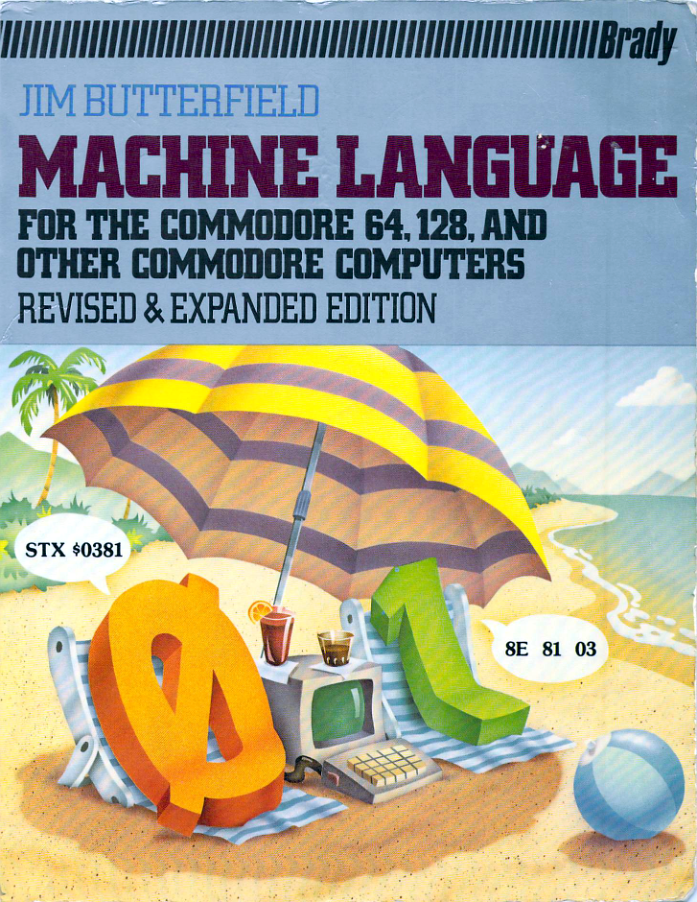
\includegraphics[width=\textwidth]{title}
\restoregeometry
%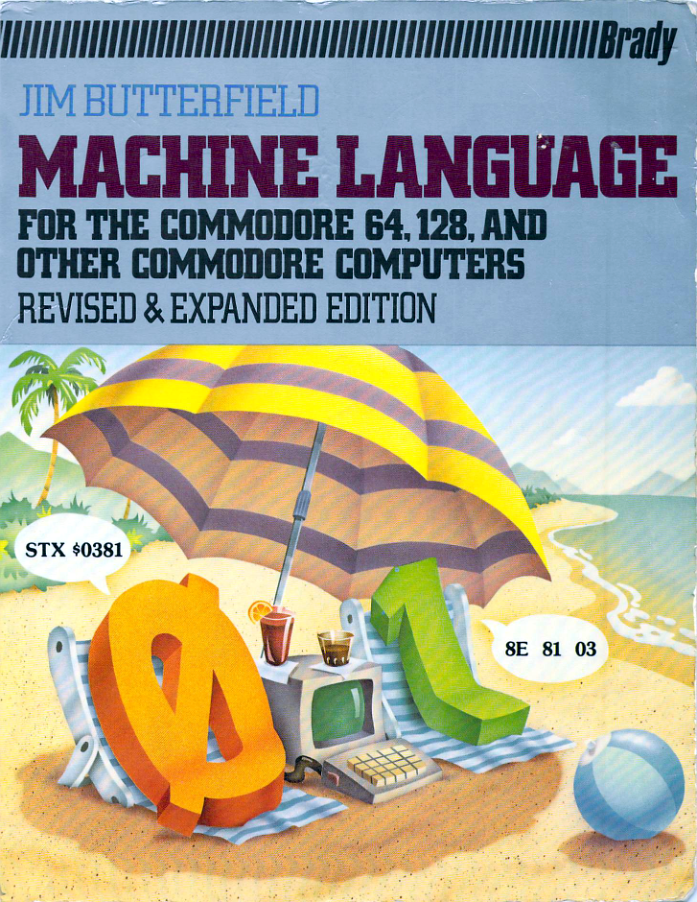
\includegraphics{title}

%\maketitle
%\newgeometry{left=2cm,right=2cm,top=2cm,bottom=2cm}
\newgeometry{margin=2cm}
\secondpage
\restoregeometry
\pagestyle{fancy}

\fancypagestyle{myfancy}{%
	\renewcommand{\headrulewidth}{1pt}%
	\renewcommand{\chaptermark}[1]{ \markboth{##1}{} }%
	\renewcommand{\sectionmark}[1]{ \markright{##1} }%
	\fancyhf{}%
	\fancyhead[LE,RO]{\thepage}%
	\fancyhead[RE]{\textit{\nouppercase{\leftmark}}}%
	\fancyhead[LO]{\textit{\nouppercase{\rightmark}}}%
}
\fancypagestyle{plain}{ %
  \fancyhf{} % remove everything
  \renewcommand{\headrulewidth}{0pt} % remove lines as well
  \renewcommand{\footrulewidth}{0pt}
}
\tableofcontents
%\listoftables
%\listoffigures
\chapter{Note to Readers}
\paragraph{}
This book introduces beginners to the principles of machine language: what it is, how it works, and how to program with it.

It is based on an intensive two-day course on machine language that has been presented many times over the past five years.

Readers of this book should have a computer on hand: students will learn by doing, not just by reading. Upon completing the tutorial material in this book, the reader will have a good idea of the fundamentals of machine language. There will be more to be learned; but by this time, students should understand how to adapt other material from books and magazines to their own particular computers.\\
\section{LIMITS OF LIABILITY AND DISCLAIMER OF WARRANTY}
\paragraph{}
The author and publisher of this book have used their best efforts in preparing this book and the programs contained in it. These efforts include the development, research, and testing of the programs to determine their effectiveness. The author and the publisher make no warranty of any kind, expressed or implied, with regard to these programs, the text, or the documentation contained in this book. The author and the publisher shall not be liable in any event for claims of incidental or consequential damages in connection with, or arising out of, the furnishing, performance, or use of the text or the programs.
\subsection{Note for Commodore 128 Owners}
\paragraph{}
The Commodore 128 is three machines in one: a Commodore 64, a Commodore 128, and a CP/M machine. You may select any of the three at any time.

If you choose the Commodore 64 mode, you'll find examples within this book that will work on your machine. The programs you write will be compatible with other (``real'') Commodore 64 computers. But you'll lose access to extra memory and to other features of the new machine. In particular, you won't have a built-in machine language monitor and will need to load one from tape or disk.

If you choose the Commodore 128 mode, you're working with a richer and more powerful machine. You will have a built-in machine language monitor for speed and convenience, and access to new features such as 80 columns, with extra complexity. There are new rules to be learned. This book contains extra material to enable you to cope with the new features of the C128.

If you choose CP/M mode, you will be in an environment that is quite different from other Commodore machines. This book, working with the 64 or 128 mode, can teach you principles of machine language and skills which may be carried to other computer environments, including CP/M. But it will not teach you CP/M itself or CP/M's machine language.

A Commodore 128 owner can read each chapter of this book twice, if desired. The first time, the exercises for the Commodore 64 can be worked through; the second time, those for the 128 can be used. The principles are the same; the code is similar; but the 128 often calls for a little more detailed work.

If you wish to learn machine language for the Commodore 128, please read the Introduction in Appendix E, under Exercises for the Commodore 128. It will give you some starting facts about your machine. There is more information on the 128 in the latter section of Appendix B and elsewhere, but don't try to read it all at the start. It will be there when you need it.
\chapter{Preface}
\paragraph{}
This book is primarily tutorial in nature. It contains, however, extensive reference material, which the reader will want to continue to use.

No previous machine language experience is required. It is useful if the reader has had some background in programming in other languages, so that concepts such as loops and decisions are understood.

Beginners will find that the material in this book moves at a fast pace. Stay with it; if necessary, skip ahead to the examples and then come back to reread a difficult
area.

Readers with some machine language experience may find some of the material too easy; for example, they are probably quite familiar with hexadecimal notation and don't need to read that part. If this is the case, skip ahead. But do enter all the programming projects; if you have missed a point, you may spot it while doing an exercise.

Programming students learn by doing. The beginner needs to learn simple things about his or her machine in order to feel in control. The elements that are needed may be itemized as:
\begin{itemize}
	\item Machine language. This is the objective, but you can't get there without the next two items.
	\item Machine architecture. All the machine language theory in the world will have little meaning unless the student knows such things as where a program may be placed in memory, how to print to the screen, or how to input from the keyboard.
	\item Machine language tools. The use of a simple machine language monitor to read and change memory is vital to the objective of making the computer do something in machine language. Use of a simple assembler and elements of debugging are easy once you know them; but until you know them, it's hard to make the machine do anything.
\end{itemize}
\paragraph{}
Principles of sound coding are important. They are seldom discussed explicitly, but run as an undercurrent through the material. The objective is this: it's easy to do things the right way, and more difficult to do them the wrong way. By introducing examples of good coding practices early, the student will not be motivated to look for a harder (and inferior) way of coding.

It should be pointed out that this book deals primarily with machine language, not assembly language. Assembler programs are marvellous things, but they are too advanced for the beginner. I prefer to see the student forming an idea of how the bytes of the program lie within memory. After this concept is firmly fixed in mind, he or she can then look to the greater power and flexibility offered by an
assembler.
\chapter{Acknowledgements}
\paragraph{}
Thanks go to Elizabeth Deal for acting as resource person in the preparation of this book. When I was hard to find, the publisher could call upon Elizabeth for technical clarification.
\chapter{Introduction}
\paragraph{}
Why learn machine language? There are three reasons. First, for speed; machine language programs are fast. Second, for versatility; all other languages are limited in some way, but not machine language. Third, for comprehension; since the computer really works in machine language only, the key to understanding how the machine operates is machine language.

Is it hard? Not really. It's finicky, but not difficult. Individual machine language instructions don't do much, so we need many of them to do a job. But each instruction is simple, and anyone can understand it if he or she has the patience.

Some programmers who started their careers in machine language find ``higher level'' languages such as BASIC quite difficult by comparison. To them, machine language instructions are simple and precise, whereas BASIC statements seem vague and poorly defined by comparison.

Where will this book take you? You will end up with a good understanding of what machine language is, and the principles of how to program in it. You won't be an expert, but you'll have a good start and will no longer be frightened by this seemingly mysterious language.

Will the skills you learn be transportable to other machines? Certainly. Once you understand the principles of programming, you'll be able to adapt. If you were to change to a non-Commodore machine that used the 6502 chip (such as Apple or Atari), you'd need to learn about the architecture of these machines and about their machine language monitors. They would be different, but the same principles would apply on all of them.

Even if you change to a computer that doesn't use a chip from the 6502 family, you will be able to adapt. As you pick through the instructions and bits of the Commodore machine, you will have learned about the principles of all binary computers. You will need to learn the new microprocessor's instruction set, but it will be much easier the second time around.

Do you need to be a BASIC expert before tackling machine language? Not at all. This book assumes you know a little about programming fundamentals: loops, branching, subroutines, and decision making. But you don't need to be an advanced programmer to learn machine language.
\newpage
\pagestyle{plain}
\begin{figure}
	\centering
	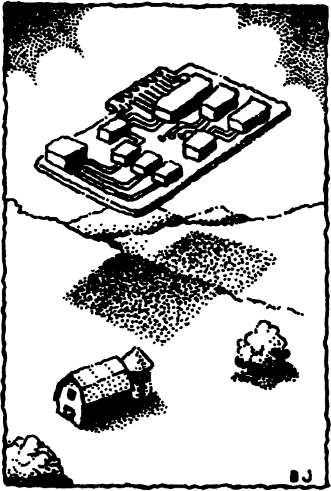
\includegraphics[width=1\linewidth]{screenshot002}
	%\caption{}
	\label{fig:screenshot002}
\end{figure}
\mainmatter
\newpage
\pagestyle{myfancy}
%\renewcommand{\headrulewidth}{1pt}%
%\renewcommand{\chaptermark}[1]{ \markboth{#1}{} }%
%\renewcommand{\sectionmark}[1]{ \markright{#1} }%
%\part{First portion}
\chapter{First Concepts}
This chapter discusses:
\begin{itemize}
	\item The inner workings of microcomputers
	\item Computer notation: binary and hexadecimal
	\item The 650x's inner architecture
	\item Beginning use of a machine language monitor
	\item A computer's ``memory layout''
	\item First machine language commands
	\item Writing and entering a simple program
\end{itemize}
\newpage
\section{The Inner Workings of Microcomputers}
All computers contain a large number of electrical circuits. Within any binary computer, these circuits may be in only two states: ``on'' or ``off.''

Technicians will tell you that ``on'' usually means full voltage on the circuit concerned, and ``off'' means no voltage. There's no need for volume control adjustments within a digital computer: each circuit is either fully on or fully off.

The word ``binary'' means ``based on two,'' and everything that happens within the computer is based on the two possibilities of each circuit: on or off. We can identify these two conditions in any of several ways:
\begin{center}
ON or OFF\\
TRUE or FALSE\\
YES or NO\\
1 or 0
\end{center}
The last description, 1 or 0, is quite useful. It is compact and numeric. If we had a group of eight circuits within the computer, some of which were ``on'' and others ``off,'' we could describe their conditions with an expression such as:\\

\texttt{11000111}\\

This would signify that the two leftmost wires were on, the next three off, and the remaining three on. The value 11000111 looks like a number; in fact, it is a binary number in which each digit is 0 or 1. It should not be confused with the equivalent decimal value of slightly over 11 million; the digits would look the same, but in decimal each digit could have a value from 0 to 9. To avoid confusion with decimal numbers, binary numbers are often preceded by a percent sign, so that the number might be shown as \texttt{\%11000111}.

Each digit of a binary number is called a bit, which is short for ``binary digit.'' The number shown above has eight bits; a group of eight bits is a byte. Bits are often numbered from the right, starting at zero. The right-hand bit of the above number would be called ``bit 0,'' and the left-hand bit would be called ``bit 7.'' This may seem odd, but there's a good mathematical reason for using such a numbering scheme.
\subsection{The Bus}
It's fairly common for a group of circuits to be used together. The wires run from one microchip to another, and then on to the next. Where a group of wires are used together and connect to several different points, the group is called a bus (sometimes spelled ``buss'').

The PET, CBM, and VIC-20 use a microprocessor chip called the 6502. The Commodore 64 uses a 6510. The Commodore B series uses a 6509 chip, and the Commodore PLUS/4 uses a chip called 7501. All these chips are similar, and there are other chips in the same family with numbers like 6504; every one works on the same principles, and we'll refer to all of them by the family name 650x.

Let's take an example of a bus used on any 650x chip. A 650x chip has little built-in storage. To get an instruction or perform a computation, the 650x must call up information from ``memory''--data stored within other chips.

The 650x sends out a ``call'' to all memory chips, asking for information. It does this by sending out voltages on a group of sixteen wires called the ``address bus.'' Each of the sixteen wires may carry either voltage or no voltage; this combination of signals is called an \emph{address}.

Every memory chip is connected to the address bus. Each chip reads the address, the combination of voltages sent by the processor. One and only one chip says, ``That's me!'' In other words, the specific address causes that chip to be selected; it prepares to communicate with the 650x. All other chips say, ``That's not me!'' and will not participate in data transfer.

\begin{figure}[h]
	\centering
	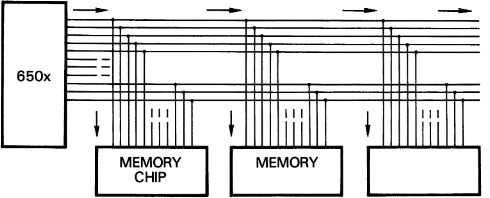
\includegraphics[width=1\linewidth]{screenshot003}
	\caption{Address bus connecting 650x \& 3 chips}
	\label{fig:screenshot003}
\end{figure}

\subsection{The Data Bus}
Once the 650x microprocessor has sent an address over the address bus and it has been recognized by a memory chip, data may flow between memory and 650x. This data is eight bits (it flows over eight wires). It might look like this:\\

\texttt{01011011}\\

The data might flow either way. That is, the 650x might \emph{read} from the memory chip, in which case the selected memory chip places information onto the data bus which is read by the microprocessor. Alternatively, the 650x might wish to \emph{write} to the memory chip. In this case, the 650x places information onto the data bus, and the selected memory chip receives the data and stores it.
\begin{figure}[h!]
	\centering
	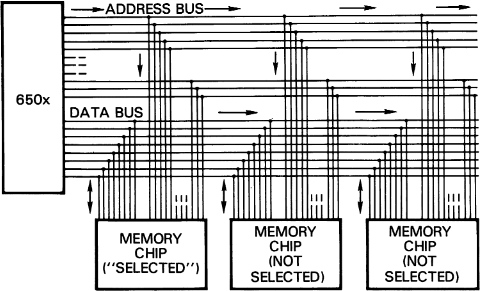
\includegraphics[width=1\linewidth]{screenshot004}
	\caption{Two-way data bus}
	\label{fig:screenshot004}
\end{figure}

All other chips are still connected to the data bus, but they have not been
selected, so they ignore the information.

The address bus is accompanied by a few extra wires (sometimes called the control bus) that control such things as data timing and the direction
in which the data should flow: read or write.
\subsection{Number Ranges}
The address bus has sixteen bits, each of which might be on or off. The
possible combinations number 65536 (two raised to the sixteenth power).
We then have 65536 different possibilities of voltages, or 65536 different
addresses.

The data bus has eight bits, which allows for 256 possibilities of voltages.
Each memory location can store only 256 distinct values.

It is often convenient to refer to an address as a decimal number. This is
especially true for PEEK and POKE statements in the BASIC language.
We may do this by giving each bit a ``weight.'' Bit zero (at the right) has
a weight of 1; each bit to the left has a weight of double the amount, so
that bit 15 (at the left) has a weight of 32768. Thus, a binary address such
as\\

\texttt{0001001010101100}\\

has a value of 4096 + 512+128 + 32 + 8 + 4 or 4780. A \texttt{POKE} to 4780
decimal would use the above binary address to reach the correct part of
memory.
\begin{figure}[h]
	\centering
	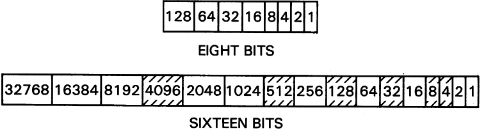
\includegraphics[width=1\linewidth]{screenshot005}
	\caption{}
	\label{fig:screenshot005}
\end{figure}

\subsection{Hexadecimal Notation}
Binary is an excellent system for the computer, but it is inconvenient for
most programmers. If one programmer asks another, ``What address should I use for some activity?'', an answer such as \texttt{``Address \%0001001010101100''} might be correct but would probably be unsatisfactory. There are too many digits.
Hexadecimal is a code used by humans to conveniently represent binary
numbers. The computer uses binary, not hexadecimal; programmers use
hexadecimal because binary is cumbersome.
To represent a binary number in hexadecimal, the bits must be grouped
together four at a time. If we take the binary value given above and split
it into groups of four, we get\\

\texttt{0001 0010 1010 1100}\\

Now each group of four bits is represented by a digit as shown in the
following table:\\

\texttt{\begin{tabular}{llll}
	0000-0 & 0100-4 & 1000-8 & 1100-C \\
	0001-1 & 0101-5 & 1001-9 & 1101-D \\
	0010-2 & 0110-6 & 1010-A & 1110-E \\
	0011-3 & 0111-7 & 1011-B & 1111-F \\
\end{tabular}}\\

Thus, the number would be represented as hexadecimal 12AC. A dollar
sign is often prefixed to a hexadecimal number so that it may be clearly
recognized:\texttt{\$12AC}.

The same type of weighting is applied to each bit of the group of four as
was described before. In other words, the rightmost bit (bit zero) has a
weight of 1, the next left a weight of 2, the next a weight of 4, and the
leftmost bit (bit three) a weight of 8. If the total of the weighted bits exceeds
nine, an alphabetic letter is used as a digit: \texttt{A} represents ten; \texttt{B}, eleven;
\texttt{C}, twelve; and \texttt{F}, fifteen.

Eight-bit numbers are represented with two hexadecimal digits. Thus,
\texttt{\%010111011} may be written as \texttt{\$5B}.
\subsection{Hexadecimal to Decimal}
As we have seen, hexadecimal and binary numbers are easily interchangeable. Although we will usually write values in ``hex,'' occasionally
we will need to examine them in their true binary state to see a particular
information bit.

Hexadecimal isn't hard to translate into decimal. You may recall that in
early arithmetic we were taught that the number 24 meant, ``two tens and
four units.'' Similarly, hexadecimal 24 means ``two sixteens and four units,''
or a decimal value of 36. By the way, it's better to say hex numbers as ``two four'' rather than ``twenty-four,'' to avoid confusion with decimal values.\\

The formal procedure, or \emph{algorithm}, to go from hex to decimal is as follows.
\begin{description}
	\item[Step 1:] Take the leftmost digit; if it's a letter \texttt{A} to \texttt{F}, convert it to the appropriate
	numeric value (\texttt{A} equals \texttt{10}, \texttt{B} equals \texttt{11}, and so on).
	\item[Step 2:] If there are no more digits, you're finished; you have the number. Stop.
	\item[Step 3:] Multiply the value so far by sixteen. Add the next digit to the result,
	converting letters if needed. Go back to step 2.
\end{description}

Using the above steps, let's convert the hexadecimal number \texttt{\$12AC}.
\begin{description}
	\item[Step 1:] The leftmost digit is \texttt{1}.
	\item[Step 2:] There are more digits, so we'll continue.
	\item[Step 3:] \texttt{1} times \texttt{16} is \texttt{16}, plus \texttt{2} gives \texttt{18}.
	\item[Step 2:] More digits to come.
	\item[Step 3:] \texttt{18} times \texttt{16} is \texttt{288}, plus \texttt{10} (for \texttt{A}) gives \texttt{298}.
	\item[Step 2:] More digits to come.
	\item[Step 3:] \texttt{298 x 16} is \texttt{4768}, plus \texttt{12} (for \texttt{C}) gives \texttt{4780}.
	\item[Step 2:] No more digits: \texttt{4780} is the decimal value.
\end{description}
This is easy to do by hand or with a calculator.
\subsection{Decimal to Hexadecimal}
The most straightforward method to convert from decimal to hexadecimal
is to divide repeatedly by 16; after each division, the remainder is the next
hexadecimal digit, working from right to left. 

This method is not too well
suited to small calculators, which usually don't give remainders. The following fraction table may offer some help:\\

\texttt{\begin{tabular}{llll}
		.0000-0 & .2500-4 & .5000-8 & .7500-C \\
		.0625-1 & .3125-5 & .5625-9 & .8125-D \\
		.1250-2 & .3750-6 & .6250-A & .8750-E \\
		.1875-3 & .4375-7 & .6875-B & .9375-F \\
\end{tabular}}\\

If we were to translate 4780 using this method, we would divide by 16, giving 298.75. The fraction tells us the last digit is \texttt{C}; we now divide 298 by 16, giving 18.625. The fraction corresponds to \texttt{A}, making the last two digits \texttt{AC}. Next we divide 18 by 16, getting 1.125 -- now the last three
digits are \texttt{2AC}. We don't need to divide the one by 16, although that would
work; we just put it on the front of the number to get an answer of \texttt{\$12AC}.

There are other methods of performing decimal-to-hexadecimal conversions. You may wish to look them up in a book on number systems. Alternatively, you may wish to buy a calculator that does the job electronically. Some programmers get so experienced that they can do conversions in their heads; I call them ``hex nuts.''

Do not get fixed on the idea of numbers. Memory locations can always
be described as binary numbers, and thus may be converted to decimal
or hexadecimal at will. But they may not \emph{mean} anything numeric: the
memory location may contain an ASCII coded character, an instruction,
or any of several other things.
\section{Memory Elements}
There are generally three types of devices attached to the memory busses
(address, data, and control busses):
\begin{itemize}
	\item \texttt{RAM}: Random access memory. This is the read and write memory, where
	we will store the programs we write, along with values used by the program.
	We may store information into \texttt{RAM}, and may recall the information at any
	time.
	\item \texttt{ROM}: Read only memory. This is where the fixed routines are kept within the
	computer. We may not store information into \texttt{ROM}; its contents were fixed 
	
	\begin{figure}[h]
		\centering
		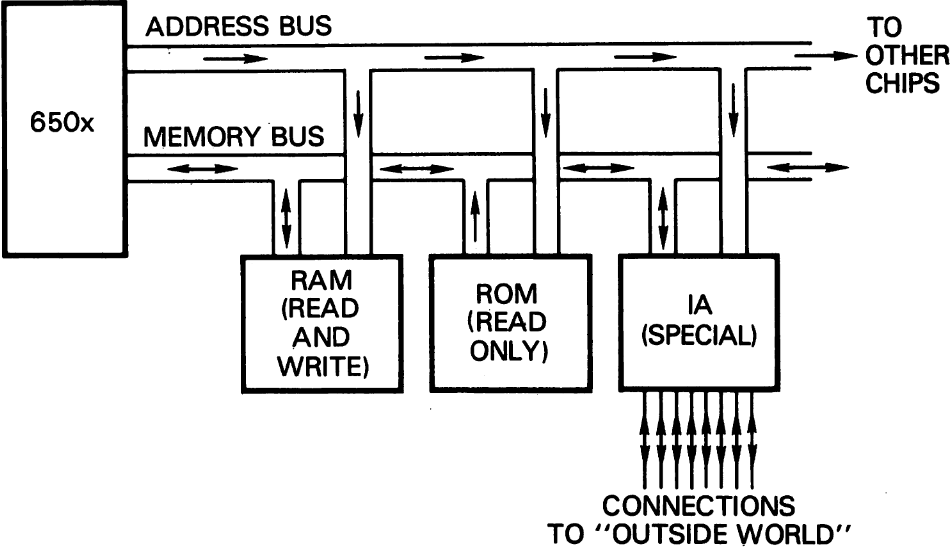
\includegraphics[width=1\linewidth]{screenshot006}
		\caption{}
		\label{fig:screenshot006}
	\end{figure}
	
	when the \texttt{ROM} was made. We will use program units (subroutines) stored in
	\texttt{ROM} to do special tasks for us, such as input and output.
	\item \texttt{IA}: Interface adaptor chips. These are not memory in the usual sense; but,
	these chips are assigned addresses on the address bus, so we call them
	``memory-mapped'' devices. Information may be passed to and from these
	devices, but the information is generally not stored in the conventional sense.
	\texttt{IA} chips contain such functions as: input/output (I/O) interfaces that serve
	as connections to the ``outside world''; timing devices; interrupt control systems; and sometimes specialized functions, such as video control or sound
	generation. IA chips come in a wide variety of designs, including the \texttt{PIA}
	(peripheral interface adaptor), the VIA (versatile interface adaptor), the \texttt{CIA}
	(complex interface adaptor), the \texttt{VIC} (video interface chip), and the \texttt{SID}
	(sound interface device).
\end{itemize}

Within a given computer, some addresses may not be used at all. Some
devices may respond to more than one address, so that they seem to be
in two places in memory.
An address may be thought of as split in two parts. One part, usually the
high part of the address, selects the specific chip. The other part of the
address selects a particular part of memory within the chip. For example,
in the Commodore 64, the hex address \texttt{\$D020} (decimal \texttt{53280}) sets
the border color of the video screen. The first part of the address (roughly,
\texttt{\$D0} ...) selects the video chip; the last part of the address (... \texttt{20})
selects the part of the chip that controls border color.

\section{Microprocessor Registers}
Within the 650x chip are several storage areas called registers. Even
though they hold information, they are not considered ``memory'' since
they don't have an address. Six of the registers are important to us. Briefly,
they are:\\

\begin{tabulary}{1.0\textwidth}{lL}
	\texttt{PC}: (16 bits) & The program counter tells where the next
	instruction will come from.\\
	\texttt{A}, \texttt{X} and t\texttt{Y} (8 bits each) &  These registers hold data.\\
	\texttt{SR} & The status register, sometimes called \texttt{PSW} (processor status word), tells about the results of recent tests, data handling, and so on.\\
	\texttt{SP} &  The stack pointer keeps track of a temporary
	storage area.\\
\end{tabulary}\\

We will talk about each of these registers in more detail later. At the
moment, we will concentrate on the PC (program counter).
\begin{figure}[h]
	\centering
	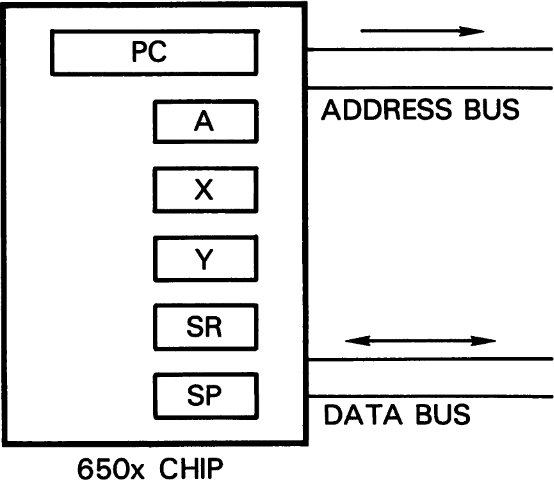
\includegraphics[width=1\linewidth]{screenshot007}
	\caption{}
	\label{fig:screenshot007}
\end{figure}

\section{Instruction Execution}
Suppose that the 650x is stopped (not an easy trick), and that there is a
certain address, say \texttt{\$1234}, in the \texttt{PC}. The moment we start the micro
computer, that address will be put out to the address bus as a read address,
and the processor will add one to the value in the \texttt{PC}.

Thus, the contents of address \texttt{\$1234} will be called for, and the \texttt{PC} will
change to \texttt{\$1235}. Whatever information comes in on the data bus will
be taken to be an \emph{instruction}.

The microprocessor now has the instruction, which tells it to do something.
The action is performed, and the whole action now repeats for the next instruction. In other words, address \texttt{\$1235} will be sent to memory, and
the \texttt{PC} will be incremented to \texttt{\$1236}.
\begin{figure}
	\centering
	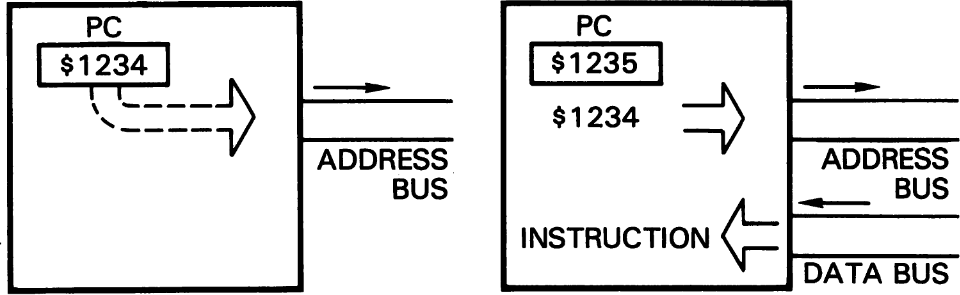
\includegraphics[width=1\linewidth]{screenshot008}
	\caption{}
	\label{fig:screenshot008}
\end{figure}

You can see that the processor works in the same way that most computer
languages do: an instruction is executed, and then the computer proceeds
to the next instruction, and then the next, and so on. We can change the
sequence of execution by means of a ``jump'' or ``branch'' to a new location,
but normally, it's one instruction after another.
\subsection{Data Registers: \texttt{A}, \texttt{X}, and \texttt{Y}}
Any of three registers can be used to hold and manipulate eight bits of
data. We may \emph{load} information from memory into \texttt{A}, \texttt{X}, or \texttt{Y}; and we may
store information into memory from any of \texttt{A}, \texttt{X}, or \texttt{Y}.

Both ``load'' and ``store'' are copying actions. If I load \texttt{A} (\texttt{LDA}) from
address \texttt{\$2345}, I make a copy of the contents of hex \texttt{2345} into A; but
\texttt{2345} still contains its previous value. Similarly, if I store \texttt{Y} into \$3456,
I make a copy of the contents of \texttt{Y} into that address; \texttt{Y} does not change.

The 650x has no way of moving information directly from one memory
address to another. Thus, this information must pass via \texttt{A}, \texttt{X}, or \texttt{Y}; we
load it from the old address, and store it to the new address.

Later, the three registers will take on individual identities. For example,
the \texttt{A} register is sometimes called the accumulator, since we perform
addition and subtraction there. For the moment, they are interchangeable:
we may load to any of the three, and we may store from any of them.
\section{First Program Project}
C128 note: The programming task that follows will need to be slightly
changed if you are using a Commodore 128 in C128 mode. In particular,
the program will need to be written into a different part of memory from
that which is shown below. Check Appendix E, Exercises for the Commodore C128, page \pageref{app:e_251} for the correct C128 coding.

Here's a programming task: locations \texttt{\$0380} and \texttt{\$0381} contain information. We wish to write a program to exchange the contents of the
two locations. How can we do this?

We must make up a plan. We know that we cannot transfer information
directly from memory to memory. We must load to a register, and then
store. But there's more. We must not store and destroy data in memory
until that data has been safely put away. How can we do this?

Here's our plan. We may load one value into \texttt{A} (say, the contents of
\texttt{\$0380}), and load the other value into \texttt{X} (the contents of \texttt{\$0381}). Then
we could store \texttt{A} and \texttt{X} back, the other way around.

We could have chosen a different pair of registers for our plan, of course:
\texttt{A} and \texttt{Y}, or \texttt{X} and \texttt{Y}. But let's stay with the original plan. We can code
our plan in a more formal way:\\

\begin{tabular}{lll}
	\texttt{LDA} & \texttt{\$0380} & (bring in first value)\\
	\texttt{LDX} & \texttt{\$0381} & (bring in second value)\\
	\texttt{STA} & \texttt{\$0381} & (store in opposite place)\\
	\texttt{STX} & \texttt{\$0380} & (and again)\\
\end{tabular}\\

You will notice that we have coded \texttt{"load A"} as \texttt{LDA}, \texttt{"load X"} as
\texttt{LDX}, \texttt{"store A"} as \texttt{STA}, and \texttt{"store X"} as \texttt{STX}. Every command
has a standard three-letter abbreviation called a \emph{mnemonic}. Had we used
the \texttt{Y} register, we might have needed to use \texttt{LDY} and \texttt{STY}.

One more command is needed. We must tell the computer to stop when
it has finished the four instructions. In fact, we can't stop the computer;
but if we use the command \texttt{BRK} (break), the computer will go to the
\emph{machine language monitor} (\texttt{MLM}) and wait for further instructions. We'll
talk about the \texttt{MLM} in a few moments.

We have written our program in a notation styled for human readability,
called \texttt{assembly language}. But the computer doesn't understand this notation. We must translate it to machine language.

The binary code for \texttt{LDA} is \texttt{\%10101101}, or hexadecimal \texttt{AD}. That's
what the computer recognizes; that's the instruction we must place in
memory. So we code the first line:\\

\begin{tabular}{llll}
	\texttt{AD 80 03} & & \texttt{LDA} & \texttt{\$0380} \\
\end{tabular}\\

It's traditional to write the machine code on the left, and the source code
on the right. Let's look closely at what has happened.

\texttt{LDA} has been translated into \texttt{\$AD}. This is the \emph{operation code}, or \emph{op code}, which says what to do. It will occupy one byte of memory. But we
need to follow the instruction with the address from which we want the
load to take place. That's address \texttt{\$0380}; it's sixteen bits long, and so
it will take two bytes to hold the address. We place the address of the
instruction, called the \emph{operand}, in memory immediately behind the instruction. But there's a twist. The last byte comes first, so that address \texttt{\$0380}
is stored as two bytes: \texttt{80} first and then \texttt{03}.

This method of storing addresses—low byte first—is standard in the 650x.
It seems unusual, but it's there for a good reason. That is, the computer
gets extra speed from this ``backwards'' address. Get used to it; you'll see
it again, many times.

Here are some machine language op codes for the instructions we may
use. You do not need to memorize them.\\

\begin{tabular}{llll}
	\texttt{LDA-AD} & \texttt{LDX-AE} & \texttt{LDY-AC} & \texttt{BRK-00} \\
	\texttt{STA-8D} & \texttt{STX-8E} & \texttt{STY-8C} &  \\
\end{tabular}\\

Now we can complete the translation of our program.\\

\texttt{\begin{tabular}{lll}
	AD 80 03 & & LDA \$0380 \\
	AE 81 03 & & LDX \$0381 \\
	8D 81 03 & & STA \$0381 \\
	8E 80 03 & & STX \$0380 \\
	00 & & BRK \\
\end{tabular}\\}

On the right, we have our plan. On the left, we have the actual program
that will be stored in the computer. We may call the right side \emph{assembly
code} and the left side \emph{machine code}, to distinguish between them. Some
users call the right-hand information \emph{source code}, since that's where we
start to plan the program, and the left-hand program \emph{object code}, since
that's the object of the exercise—to get code into the computer. The job
of translating from source code to object code is called \emph{assembly}. We
performed this translation by looking up the op codes and translating by
hand; this is called \emph{hand assembly}.

The code must be placed into the computer. It will consist of 13 bytes:
\texttt{AD 80 03 AE 81 03 8D 81 03 8E 80 03 00}. That's the
whole program. But we have a new question: where do we put it?
\subsection{Choosing a Location}
We must find a suitable location for our program. It must be placed into
\texttt{RAM} memory, of course, but where?

For the moment, we'll place our program into the cassette buffer, starting
at address \texttt{\$033C} (decimal \texttt{828}). That's a good place to put short test programs, which is what we will be writing for a while.

Now that we've made that decision, we face a new hurdle: how do we get
the program in there? To do that, we need to use a machine language
monitor.
\section{Monitors: What They Are}
All computers have a built-in set of programs called an \emph{operating system}
that gives the machine its style and basic capabilities. The operating system takes care of 
communications—reading the keyboard, making the
proper things appear on the screen, and transferring data between the
computer and other devices, such as disk, tape, or printer.

When we type on the computer keyboard, we use the operating system,
which detects the characters we type. But there's an extra set of programs
built into the computer that must decide what we \emph{mean}. When we are
using the BASIC language, we'll be communicating with the BASIC monitor, which understands BASIC commands such as \texttt{NEW}, \texttt{LOAD}, \texttt{LIST},
or \texttt{RUN}. It contains editing features that allow us to change the BASIC
program that we are writing.

But when we switch to another system—often another language—we'll
need to use a different monitor. Commands such as \texttt{NEW} or \texttt{LIST} don't
have any meaning for a machine language program. We must leave the
BASIC monitor and enter a new environment: the \emph{machine language monitor}. We'll need to learn some new commands because we will be communicating with the computer in a different way.

\section{The Machine Language Monitor}
Most PET/CBM computers have a simple \texttt{MLM} (machine language monitor) 
built in. It may be extended with extra commands. The Commodore
PLUS/4 contains a very powerful \texttt{MLM}. The VIC-20 and Commodore 64
do not have a built-in \texttt{MLM}, but one can be added. Such a monitor may
be either loaded into RAM or plugged in as a cartridge. Monitors may be
purchased or obtained from user clubs.

Most machine language monitors work in a similar way, and have about
the same commands. To proceed, you'll need an \texttt{MLM} in your computer.
Use the built-in one, plug it in, load it in, or load and run ... whatever the
instructions tell you. On a PET/CBM machine, typing the command \texttt{SYS
4} will usually switch you to the built-in monitor After an \texttt{MLM} has been
added to a VIC or Commodore 64, the command \texttt{SYS 8} will usually get
you there. On the Commodore PLUS/4, the BASIC command \texttt{MONITOR}
will bring the monitor into play.

C128 note: When the Commodore 128 is in C64 mode, it needs to have
a monitor program loaded, as does the Commodore 64. When in the C128
mode, however, the command \texttt{MONITOR} will bring the monitor into play.
There will be slight differences in the screen display of this monitor.
Appendix H contains information on the various monitor commands and
formats.

Caution: Occasionally, you may run across a monitor which uses—and
changes—memory locations in the address range \texttt{\$033C} to \texttt{\$03F0},
which is where we will put many of our programs. There is a version of
program MICROMON which does this. Such a monitor will create problems
for us as we try to work the following examples, since our programs and
data will be changed by the monitor as we use it. The built-in monitors
will certainly not have any problem. If you encounter any problems with
the following examples, and it appears that your program is being mysteriously
changed, switch to another machine language monitor.
\subsection{Monitor Display}
The moment you enter the MLM, you'll see a display that looks something
like this:\\

\texttt{\begin{tabular}{ccccccc}
	B* &  &  &  &  &  &  \\
	& PC & SR & AC & XR & YR & SP \\
	& 0005 & 20 & 54 & 23 & 6A & F8 \\
\end{tabular}\\}

The cursor will be flashing to the right of the period on the bottom line.
The exact appearance of the screen information may vary according to
the particular monitor you are using. Other material may be displayed—
in particular, a value called \texttt{IRQ}—which we will ignore for the time being.\\

The information you see may be interpreted as follows:
\begin{description}
	\item[\texttt{B*}] we have reached the \texttt{MLM} by means of a ``break.'' More about that later.
	\item[\texttt{PC}] The value shown below this title is the contents of the program counter.
	This indicates where the program ``stopped.'' In other words, if the value shown
	is address 0005, the program stopped at address \texttt{0004}, since the PC is
	ready to continue at the following address. The exact value (\texttt{0004} versus
	\texttt{0005}) may vary depending on the particular \texttt{MLM}.
	\item[\texttt{SR}] The value shown below shows the status register, which tells us the results
	of recent tests and data operations. We'd need to split apart the eight bits and
	look at them individually to establish all the information here; we will do this at
	a later time.
	\item[\texttt{AC}, \texttt{XR} and \texttt{YR}] The values shown below these three titles are the contents
	of our three data registers: \texttt{A}, \texttt{X}, and \texttt{Y}.
	\item[\texttt{SP}] The value shown below is that of the stack pointer, which indicates a
	temporary storage area that the program might use. A value of \texttt{F8}, for example,
	tells us that the next item to be dropped into the stack area would go to address
	\texttt{\$01F8} in memory. More on this later.
\end{description}

You will notice that the display printed by the monitor (called the register
display) shows the internal registers within the 650x chip. Sometimes there
is another item of information, titled \texttt{IRQ}, in this display. It doesn't belong,
since it does not represent a microprocessor register. \texttt{IRQ} tells us to what
address the computer will go if an \emph{interrupt} occurs; this information is
stored in memory, not within the 650x.
\section{MLM Commands}
\blindtext
\section{Changing Memory Contents}
\blindtext
\section{Changing Registers}
\blindtext
\section{Entering the Program}
\blindtext
\section{Things You Have Learned}
\blindtext
\section{Detail: Program Execution}
\blindtext
\section{Questions and Projects}
\blindtext
\chapter{Controlling Output}
\blindtext
\newpage
\section{Calling Machine Language Subroutines}
\blindtext
\section{CHROUT—The Output Subroutine}
\blindtext
\section{Why Not POKE?}
\blindtext
\section{A Print Project}
\blindtext
\section{Monitor Extensions}
\blindtext
\section{Checking: The Disassembler}
\blindtext
\section{Running the Program}
\blindtext
\section{Linking with BASIC}
\blindtext
\section{Loops}
\blindtext
\section{Things You Have Learned}
\blindtext
\section{Questions and Projects}
\blindtext
\chapter{Flags, Logic, and Input}
\blindtext
\newpage
\section{Flags} 
\blindtext
\section{A Brief Diversion: Signed Numbers} 
\blindtext
\section{A Brief Diversion: Overflow} 
\blindtext
\section{Flag Summary} 
\blindtext
\section{The Status Register} 
\blindtext
\section{Instructions: A Review} 
\blindtext
\section{Logical Operators} 
\blindtext
\section{Why Logical Operations?} 
\blindtext
\section{Input: The GETIN Subroutine} 
\blindtext
\section{STOP} 
\blindtext
\section{Programming Project} 
\blindtext
\section{Things You Have Learned} 
\blindtext
\section{Questions and Projects} 
\blindtext
\appendix
\part{Appendix}
\chapter{The 6502/6510/6509/7501/8500 Instruction Set}
\section{Addressing Modes}
\blindtext
\chapter{Some Characteristics of Commodore Machines}
\blindtext
\chapter{Memory Maps}
\blindtext
\chapter{Character Sets}
\blindtext
\chapter{Exercises for Alternative Commodore Machines}
%\label{app:e}
\label{app:e_251}
\blindtext
\chapter{Floating Point Representation}
\blindtext
\chapter{Uncrashing}
\blindtext
\chapter{Supermon Instructions}
\blindtext
\chapter{IA Chip Information}
\blindtext
\chapter{Disk User's Guide}
\blindtext
\end{document}
